% !TeX root = ../main.tex

\chapter{案例分析}

本章為案例分析,以整合了一座假想風力電場與電動汽車的虛擬電廠為研究對象,詳述完整的分析過程與使用條件。內容可大致分為三個部分,第一部分說明計算設備規格、資料來源與模擬情境;第二部分進行短期風速預測,計算不同預測模型的誤差結果來比較模型的預測能力;第三部分進行收益結果分析,分別針對不同參數下的結果進行討論。

\section{模擬情境概述}

% 設備概述
本研究使用 Python 程式語言及開源數值分析與統計模型套件 \texttt{pyramid}、\texttt{sklearn} 和 \texttt{pywt} 等實作短期風速預測部分,搭配 MathWorks 公司出品的商業數學軟體 $\text{MATLAB}^{®}$ 中的模型預測控制工具箱 (Model Predictive Control Toolbox™) 和動態系統模擬軟體 $\text{Simulink}^{®}$ 進行收益模型規劃求解。進行模擬與分析所使用的計算設備,其硬體規格採用 $\text{Intel}^{®}$ $\text{Xeon}^{®}$ E5-2620 處理器,記憶體共 $64$ GB 並運行 Ubuntu 18.04 LTS 作業系統。

% 風力資料
歷史風速資料與模擬場址的選擇,考量我國\uline{澎湖}、\uline{金門}與\uline{馬祖}地區等離島地區由於孤立於臺灣本島的電力傳輸系統之外,較適合作為含風力發電與電動汽車的虛擬電廠參與電力市場交易的模擬案例。本研究使用\uline{東吉島} (DONGJIDAO) 氣象測站 (北緯 $23^\circ 15' 32''$,東經 $119^\circ 39'34''$) 於 2018 年的風速資料,並根據表 \ref{table: Taiwan Wind Farm Data} 所示的我國風力發電場址資料,假設模型中的風力電場由八座 Enercon E40/600 Model 風力發電機組與六座 Enercon E44/900 Model 風力發電機組所構成。

% 電力價格
收益分析部分的電力價格,考慮未來電力市場自由化將使發電業者跳脫政府以特定費率在特定年限收購電力的躉購 (Feed-In Tariff, FIT) 制度擁抱自由市場,本研究採用因應不同用電狀況與發電情況所制定的時間電價 (Time of Use Tariff, TOU) 方案,這樣一來虛擬電廠在參與電力市場交易時,可以根據時間電價進行儲能設備的調度,用以平衡波動並獲取較大收益,比如在電價較低的離峰時段儲存電能至電動汽車或儲能設備中,而在電價較高的尖峰時端販售電力。目前由於我國智慧電錶尚未完全普及,未能有效針對不同時段制定電價,而是以季節區分並制定兩段式或三段式浮動電價,本文採用表 \ref{table: Electric Price} 所示的\uline{臺灣}電力公司非夏季兩段式電價進行收益計算 \cite{taipower2018price}。

\begin{table}[htbp]
  \centering
  \caption[臺灣電力公司非夏季兩段式電價]{臺灣電力公司非夏季的兩段式電價 \cite{taipower2018price}}
  \begin{tabular}{cr}
    \toprule
    \textbf{時間區段} & \textbf{電力價格 (NT/度) } \\
    \midrule
    00:00 - 07:30 & NT \$1.73 \\
    07:30 - 22:30 & NT \$4.23 \\
    22:30 - 24:00 & NT \$1.73 \\
    \bottomrule
  \end{tabular}
  \label{table: Electric Price}
\end{table}

% 電動汽車
研究中用於估算的電動汽車,採用美國特斯拉汽車公司於 2018 年所推出的 Model 3 車款,其電池容量根據所選配置介於 $54$ \si{\kWh}  (Standard Range) 至 $79$ \si{\kWh}  (Long Range) 之間,本研究設置電動汽車電池容量為標準款的 $54$ \si{\kWh}。另外根據 2018 年美國能源局的研究報告所提供之資料,該年度電動車轉換的效率可達 $77\%$ 至 $82\%$,因此本研究採用之電池能源轉換損耗比例為 $\eta = 0.23$。

\section{短期風速預測}

\subsection{風速資料取得}

受限於風力電場的風速資料僅為營運商所持有,本文中於風力發電數量預測部分所使用的歷史風速,採用該地區的氣象觀測資料,目前\uline{臺灣}地區各氣象測站的觀測資料可以透過中央氣象局的觀測資料查詢系統 (CWB Observation Data Inquire System, CODiS) 進行查詢,僅需選定測站位置與日期並指定資料格式,即可獲取包含風速、風向、降水量、日照時數等資料。

\subsection{歷史風速概述}

此處採用\uline{東吉島} (DONGJIDAO) 測站於 $2018$ 年間風速跨度較大的十二月份歷史風速進行短期風速預測預測範例計算,取該月份中前二十九日共 $696$ 個小時的歷史風速作為觀測資料,預測最後二日共 $48$ 小時的短期風速,並比較不同預測模型的誤差結果。在後續內容中,將選擇預測能力較佳的模型來預測收益分析中風力電場的發電數量。

圖 \ref{figure: Historial Wind Speed} 為根據\uline{東吉島} (DONGJIDAO) 測站 $2018$ 年十二月份的歷史風速資料所繪製的原始風速時間序列,顯示在該月份中所測得之歷史風速有較大幅度的變化,且初步判斷該時間序列具備一定的趨勢性,可能為一非平穩時間序列。

\begin{figure}[htbp]
  \centering
  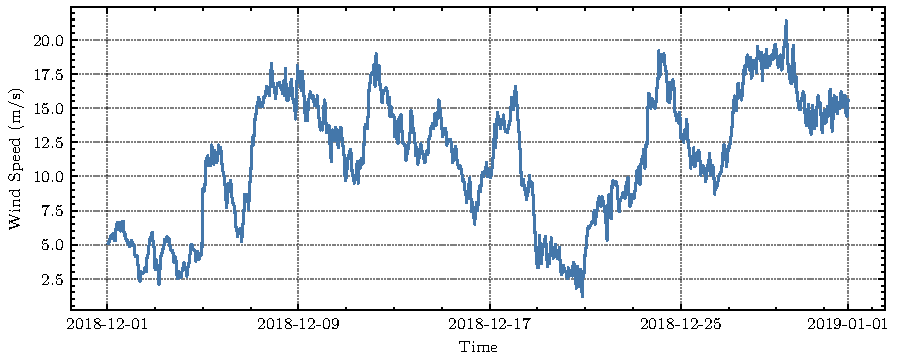
\includegraphics[width=\textwidth]{Historial Wind Speed}
  \caption{原始風速時間序列}
  \label{figure: Historial Wind Speed}
\end{figure}

由於採用圖形檢驗法觀察時間序列平穩性可能根據觀察者不同而存在主觀性差異,本文採用 Augmented Dickey-Fuller 檢定進行單根檢驗,其平穩性檢驗結果如表 \ref{table: Raw Time Series ADF Result} 所示,由於 ADF 檢驗統計量並不同時小於在 $99\%$、$95\%$ 與 $90\%$ 信賴區間下的 ADF 臨界檢驗值,因此原始風速資料時間序列為非平穩時間序列。

\begin{table}[htbp]
  \centering
  \caption[原始風速時間序列 ADF 檢定結果]{原始風速時間序列 ADF 檢定結果}
  \begin{tabular}{lr}
    \toprule
    \textbf{檢驗統計量}     & \textbf{結果} \\
    \midrule
    Test Statistic          & $-3.217446$ \\
    p-value                 & $1.8997 \times 10^{-2}$ \\
    Critical Value ($1\%$)  & $-3.439377$ \\
    Critical Value ($5\%$)  & $-2.865524$ \\
    Critical Value ($10\%$) & $-2.568891$ \\
    \bottomrule
  \end{tabular}
  \label{table: Raw Time Series ADF Result}
\end{table}

\subsection{單一預測模型}

\subsubsection{ARIMA 預測模型}

由於 ARIMA 模型的概念在於透過歷史資料的自相關性進行未來結果的預測,為使採用樣本時間序列所得到的擬合曲線在未來短期時間內延續既有型態,所採用的時間序列須具備平穩性。由前述內容已知原始風速時間序列為非平穩時間序列,因此需反覆計算時間序列中當前時刻與前一時刻的差值來取得其差分後的平穩時間序列。

\begin{figure}[htbp]
  \centering
  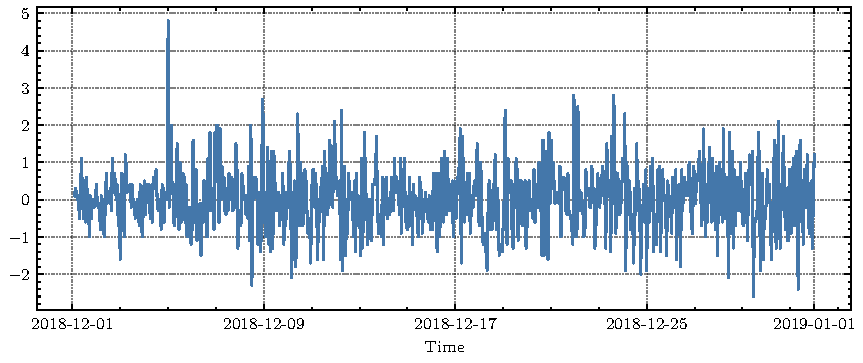
\includegraphics[width=\textwidth]{Difference Wind Speed}
  \caption{差分風速時間序列}
  \label{figure: Difference Wind Speed}
\end{figure}

將原始風速時間序列進行一階差分後所得到的差分風速時間序列如圖 \ref{figure: Difference Wind Speed} 所示,由圖形可初步判斷該時間序列已具備平穩性。為避免觀察者不同而存在的主觀性差異,採用 Augmented Dickey-Fuller 檢定進行單根檢驗的平穩性檢驗結果如表 \ref{table: Difference Time Series ADF Result} 所示,其中 ADF 檢驗統計量已同時小於在 $99\%$、$95\%$ 與 $90\%$ 信賴區間下的 ADF 臨界檢驗值,且 p-value 已十分接近零,因此該差分風速時間序列已為平穩時間序列。

\begin{table}[htbp]
  \centering
  \caption[差分風速時間序列 ADF 檢定結果]{差分風速時間序列 ADF 檢定結果}
  \begin{tabular}{lr}
    \toprule
    \textbf{檢驗統計量}     & \textbf{Value}             \\
    \midrule
    Test Statistic          & $-21.391265$               \\
    p-value                 & $5.817483 \times 10^{-27}$ \\
    Critical Value ($1\%$)  & $-3.439206$                \\
    Critical Value ($5\%$)  & $-2.865448$                \\
    Critical Value ($10\%$) & $-2.568851$                \\
    \bottomrule
  \end{tabular}
  \label{table: Difference Time Series ADF Result}
\end{table}

圖 \ref{figure: Difference Wind Speed ACF} 和圖 \ref{figure: Difference Wind Speed PACF} 分別為差分時間序列的自相關函數 (Autocorrelation Function, ACF) 圖與非自相關函數 (Partial Autocorrelation Function, PACF) 圖,由圖形可知其自相關函數在延遲項 Lag 值為 $2$ 時落入信賴區間中,其偏自相關函數在延遲項 Lag 值為 $3$ 時落入信賴區間中,據此可認定其時間序列具備平穩性並可大致識別其模型可採用 $\text{ARIMA} (2, 1, 3)$。

\begin{figure}[htbp]
  \centering
  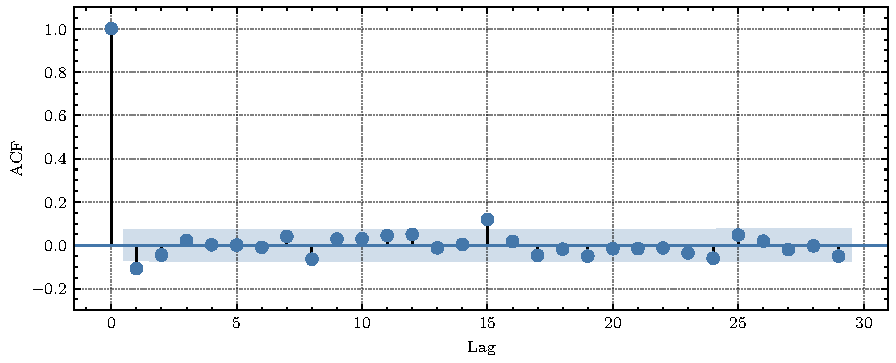
\includegraphics[width=\textwidth]{Difference Wind Speed ACF}
  \caption{差分時間序列自相關函數 (ACF) 圖}
  \label{figure: Difference Wind Speed ACF}
\end{figure}

\begin{figure}[htbp]
  \centering
  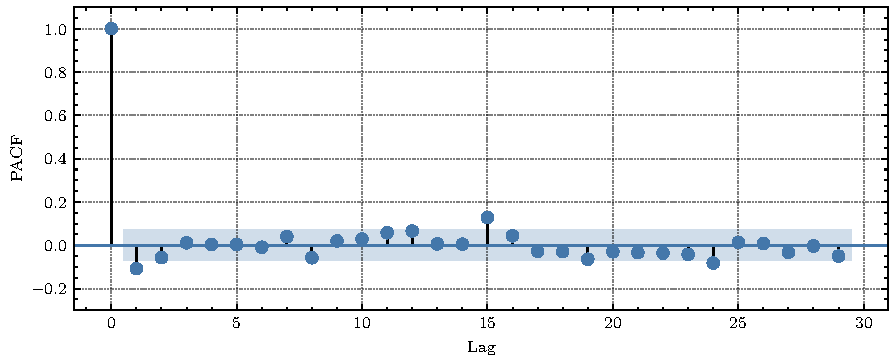
\includegraphics[width=\textwidth]{Difference Wind Speed PACF}
  \caption{差分時間序列偏自相關函數 (PACF) 圖}
  \label{figure: Difference Wind Speed PACF}
\end{figure}

透過自相關函數圖與偏自相關函數圖進行模型定階可能存在主觀性差異,通常會使用赤池資訊準則 (Akaike's Information Criterion, AIC) 及貝氏資訊準則 (Bayesian Information Criterion, BIC) 作為評價模型優劣的指標,採用窮舉法擬合所有模型並選出具有較小 AIC 值的最適模型。表 \ref{table: Auto ARIMA Result} 為使用開源統計套件 \texttt{pyramid} 所提供的 \texttt{auto\_arima()} 函數針對差分時間序列模型進行窮舉擬合所得到的結果,最終採用 AIC 值最小的 $\text{ARIMA} (2, 1, 0)$ 模型進行短期預測,預測結果如圖 \ref{figure: Wind Speed Prediction ARIMA} 所示。

\begin{table}[htbp]
  \centering
  \caption[差分風速時間序列 $\text{ARIMA}(p, d, q)$ 適配檢驗]{差分風速時間序列 $\text{ARIMA}(p, d, q)$ 適配檢驗}
  \begin{tabular}{cccc}
    \toprule
    \textbf{\text{ARIMA}(p, d, q)} & \textbf{AIC} & \textbf{BIC} & \textbf{Time} \\
    \midrule
    $\text{ARIMA}(1,1,1)$ & $1886.365$ & $1904.808$ & $0.229$ \si{s} \\
    $\text{ARIMA}(1,1,2)$ & $1886.528$ & $1909.581$ & $0.424$ \si{s} \\
    $\text{ARIMA}(1,1,3)$ & $1888.300$ & $1915.964$ & $0.404$ \si{s} \\
    $\text{ARIMA}(1,1,4)$ & $1890.242$ & $1922.517$ & $0.619$ \si{s} \\
    $\text{ARIMA}(2,1,0)$ & $1885.681$ & $1904.124$ & $0.087$ \si{s} \\
    $\text{ARIMA}(2,1,1)$ & $1887.588$ & $1910.641$ & $0.258$ \si{s} \\
    $\text{ARIMA}(2,1,2)$ & $1889.564$ & $1917.228$ & $0.165$ \si{s} \\
    $\text{ARIMA}(2,1,3)$ & $1890.281$ & $1922.556$ & $0.890$ \si{s} \\
    $\text{ARIMA}(3,1,0)$ & $1887.576$ & $1910.630$ & $0.110$ \si{s} \\
    $\text{ARIMA}(3,1,1)$ & $1889.572$ & $1917.236$ & $0.155$ \si{s} \\
    $\text{ARIMA}(3,1,2)$ & $1890.944$ & $1923.219$ & $0.955$ \si{s} \\
    $\text{ARIMA}(4,1,0)$ & $1889.565$ & $1917.229$ & $0.138$ \si{s} \\
    $\text{ARIMA}(4,1,1)$ & $1891.564$ & $1923.839$ & $0.184$ \si{s} \\
    \bottomrule
  \end{tabular}
  \label{table: Auto ARIMA Result}
\end{table}

\begin{figure}[h]
  \centering
  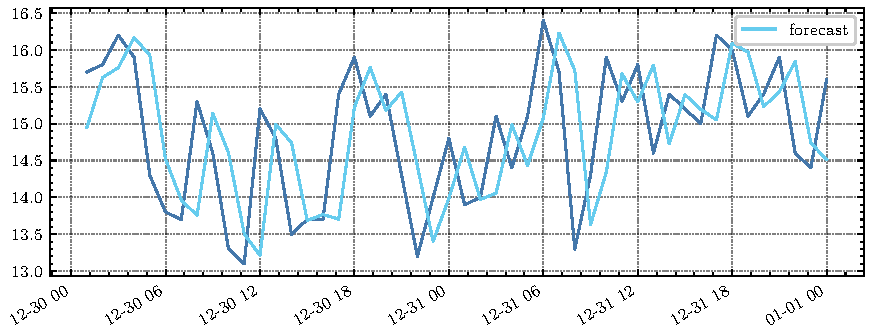
\includegraphics[width=\textwidth]{Wind Speed Prediction (ARIMA)}
  \caption{單一 ARIMA 模型短期風速預測結果}
  \label{figure: Wind Speed Prediction ARIMA}
\end{figure}

\subsubsection{SVR 預測模型}

使用支持向量迴歸模型進行時間序列預測時,在將歷史風速資料進行標準化後,採用時間間隔為 $1$ 單位的延遲,並選用高斯徑向核函數進行預測。使用開放式源代碼套件 \texttt{sklearn} 所提供的 \texttt{SVR()} 函數針對風速時間序列模型進行預測的結果如圖 \ref{figure: Wind Speed Prediction SVR} 所示。

\begin{figure}[h]
  \centering
  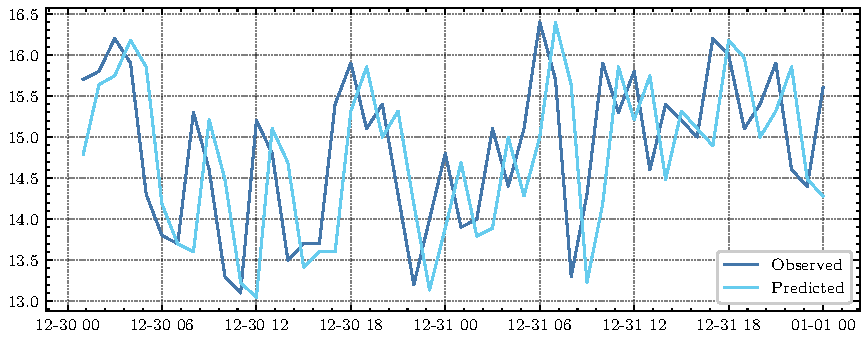
\includegraphics[width=\textwidth]{Wind Speed Prediction (SVR)}
  \caption{單一 SVR 模型短期風速預測結果}
  \label{figure: Wind Speed Prediction SVR}
\end{figure}

\subsection{組合預測模型}

\subsubsection{一般等權 ARIMA-SVR 組合模型}

本文採用的一般等權 ARIMA-SVR 組合模型如方程式 \eqref{equation: Normal Combine Model} 所示,即使用相等權重將前述單一預測模型中 ARIMA 模型與 SVR 模型的預測結果進行線性組合。根據單一 ARIMA 模型與單一 SVR 模型預測結果進行相等權重線性組合的預測結果如圖 \ref{figure: Wind Speed Prediction Linear} 所示。

\begin{figure}[h]
  \centering
  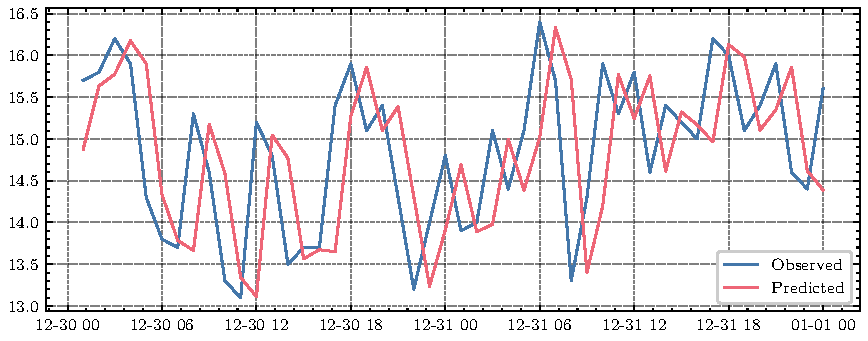
\includegraphics[width=\textwidth]{Wind Speed Prediction (Linear)}
  \caption{一般等權 ARIMA-SVR 組合模型短期風速預測結果}
  \label{figure: Wind Speed Prediction Linear}
\end{figure}

\subsubsection{小波分解 ARIMA-SVR 組合模型}

本文採用的小波分解 ARIMA-SVR 組合模型如方程式 \eqref{equation: Wavelet Combine Model} 所示,即將時間序列透過離散小波轉換分解為近似分量與細節分量,並分別採用 ARIMA 模型預測與 SVR 模型預測,再將預測結果進行重構與整合。

針對時間序列採用較平滑且解析度較高的 Daubechies Wavelet 小波或 Symlet 小波進行分解較為合適。本文先使用不同消失矩 $N$ 的 Daubechies Wavelet 小波將原始風速時間序列進行不同層數的訊號分解後,再進行訊號重構所得到的誤差如表 \ref{table: Wavelet Reconstruction Error} 所示,顯示採用 db4 小波進行 $2$ 層的訊號分解能夠在訊號重構時產生較小的誤差。

\begin{table}[htbp]
  \centering
  \caption[原始風速時間序列進行小波分解的重構誤差]{原始風速時間序列進行小波分解的重構誤差}
  \begin{tabular}{lcccc}
    \toprule
    \textbf{分解層數} & $\text{db}_3$ \textbf{小波} & $\text{db}_4$ \textbf{小波} & $\text{db}_5$ \textbf{小波} & $\text{db}_6$ \textbf{小波} \\
    \midrule
    $2$ 層分解 & $2.8931$ & $1.1759$ & $4.2143$ & $3.2171$ \\
    $3$ 層分解 & $4.1932$ & $2.1486$ & $5.9631$ & $4.7622$ \\
    $4$ 層分解 & $4.3194$ & $3.0123$ & $7.3174$ & $5.4318$ \\
    \bottomrule
    & & & & ($\times 10^{-10}$)
  \end{tabular}
  \label{table: Wavelet Reconstruction Error}
\end{table}

在使用開放式源代碼套件 \texttt{pywt} 所提供的 \texttt{wavedec()} 函數,選擇 db4 小波對原始風速時間序列進行 $2$ 層小波分解與重構後,可以得到如圖 \ref{figure: Approximated Component Level 2 (A2)} 所示反映整體趨勢的近似分量 $\text{A}_2$,以及如圖 \ref{figure: Detailed Component Level 2 (D2)} 和圖 \ref{figure: Detailed Component Level 1 (D1)} 所示反映細小波動的細節分量 $\text{D}_2$ 和 $\text{D}_1$。

\begin{figure}[hbp]
  \centering
  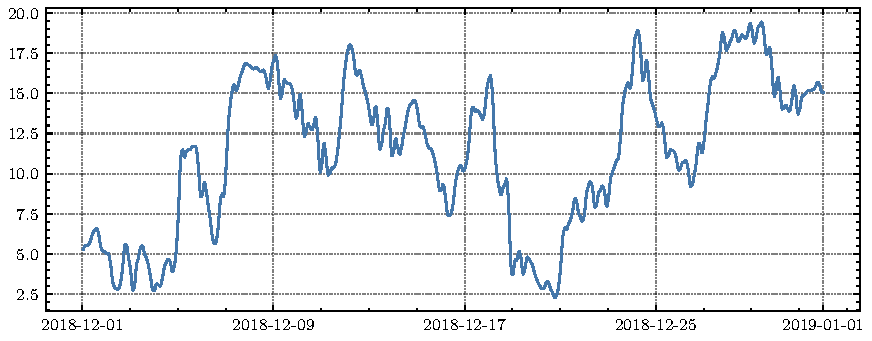
\includegraphics[width=\textwidth]{Approximated Component in Level 2 (A2)}
  \caption{原始風速時間序列進行小波分解的近似分量 $\text{A}_2$}
  \label{figure: Approximated Component Level 2 (A2)}
  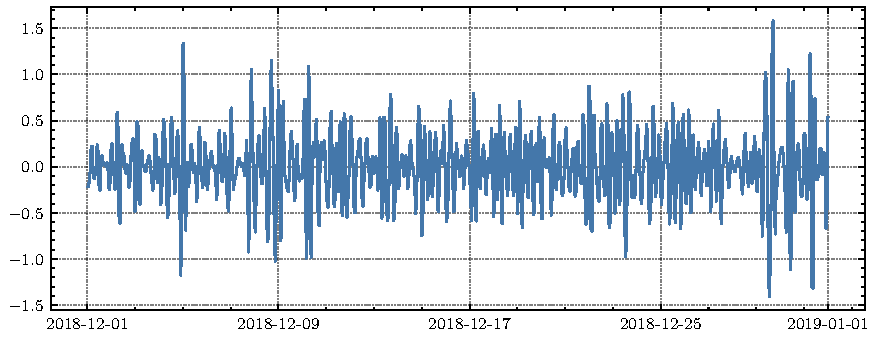
\includegraphics[width=\textwidth]{Detailed Component in Level 2 (D2)}
  \caption{原始風速時間序列進行小波分解的細節分量 $\text{D}_2$}
  \label{figure: Detailed Component Level 2 (D2)}
  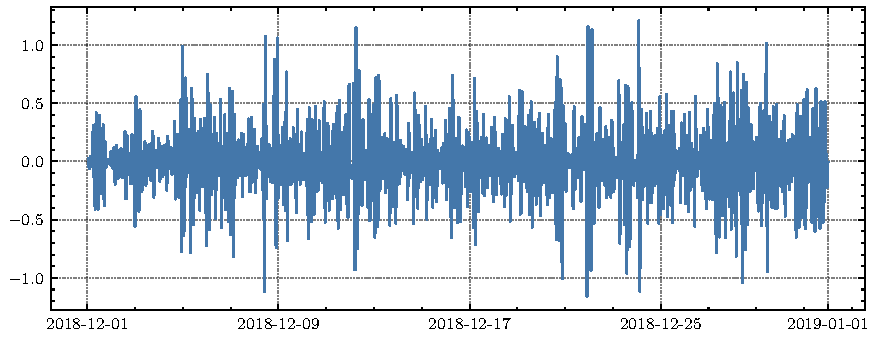
\includegraphics[width=\textwidth]{Detailed Component in Level 1 (D1)}
  \caption{原始風速時間序列進行小波分解的細節分量 $\text{D}_1$}
  \label{figure: Detailed Component Level 1 (D1)}
\end{figure}

採用 Augmented Dickey-Fuller 檢定對原始風速時間序列經小波分解後所得到的近似分量 $\text{A}_2$ 進行單根檢驗,其平穩性檢驗結果如表 \ref{table: A2 ADF Result} 所示,其 ADF 檢驗統計量並不同時小於在 $99\%$、$95\%$ 與 $90\%$ 信賴區間下的 ADF 臨界檢驗值,因此該近似分量時間序列為非平穩時間序列。

\begin{table}[htbp]
  \centering
  \caption[原始風速時間序列 $\text{A}_2$ 近似分量 ADF 檢定結果]{原始風速時間序列 $\text{A}_2$ 近似分量 ADF 檢定結果}
  \begin{tabular}{lr}
    \toprule
    \textbf{檢驗統計量}     & \textbf{結果} \\
    \midrule
    Test Statistic          & $-2.490732$ \\
    p-value                 & $0.117746$ \\
    Critical Value ($1\%$)  & $-3.439402$ \\
    Critical Value ($5\%$)  & $-2.865535$ \\
    Critical Value ($10\%$) & $-2.568897$ \\
    \bottomrule
  \end{tabular}
  \label{table: A2 ADF Result}
\end{table}

如同前述步驟,需針對近似分量 $\text{A}_2$ 進行差分平穩化,並進行窮舉擬合後,選用 $\text{ARIMA} (2, 1, 2)$ 模型進行預測,並對細節分量 $\text{D}_2$ 與 $\text{D}_1$ 分別採用向量迴歸模型進行預測。最後將兩者預測結果進行整合可得到小波分解 ARIMA-SVR 組合模型的短期風速預測結果如圖 \ref{figure: Wind Speed Prediction Wavelet} 所示。

\begin{figure}[htbp]
  \centering
  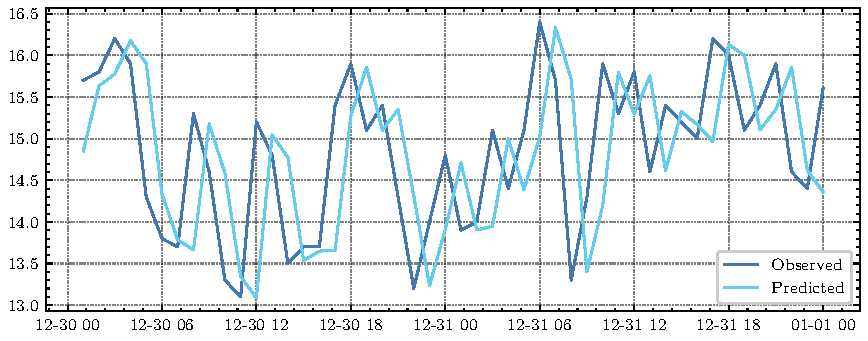
\includegraphics[width=\textwidth]{Wind Speed Prediction (Wavelet)}
  \caption{小波分解 ARIMA-SVR 組合模型短期風速預測結果}
  \label{figure: Wind Speed Prediction Wavelet}
\end{figure}

\subsection{模型誤差比較}

為比較在短期風速預測中採用小波分解 ARIMA-SVR 組合模型是否相較傳統單一預測模型具有較好的效果,本文使用同一段時間內的歷史風速資料,分別採用了單一 ARIMA 預測模型、單一 SVR 預測模型、一般等權 ARIMA-SVR 組合模型與小波分解 ARIMA-SVR 組合模型進行預測。計算其平均絕對百分比誤差 (MAPE) 、平均絕對誤差 (MAE) 與均方根誤差 (RMSE) 作為模型優劣的評價依據,結果如表 \ref{table: Time Series Model Result} 所示。

\begin{table}[htbp]
  \centering
  \caption[風速預測模型評估結果]{風速預測模型評估結果}
  \begin{tabular}{lccc}
    \toprule
    \textbf{Model}              & \textbf{MAPE} & \textbf{MAE} & \textbf{RMSE} \\
    \midrule
    單一 ARIMA 預測模型         & $5.2838 \%$   & $0.7788$     & $0.9654$ \\
    單一 SVR 預測模型           & $5.4723 \%$   & $0.8113$     & $0.9869$ \\
    一般等權 ARIMA-SVR 組合模型 & $5.3688 \%$   & $0.7938$     & $0.9730$ \\
    小波分解 ARIMA-SVR 組合模型 & $5.1482 \%$   & $0.7591$     & $0.9418$ \\
    \bottomrule
  \end{tabular}
  \label{table: Time Series Model Result}
\end{table}

結果顯示,短期風速的預測模型中,不論是採用 ARIMA 時間序列預測模型或是向量支持回歸預測,在使用平均絕對百分比誤差 (MAPE) 、平均絕對誤差 (MAE) 與均方根誤差 (RMSE) 作為模型優劣的評價依據下皆有不錯的預測效果,而又以前者的預測能力較好。而在使用小波分解將原始時間序列訊號分解之後,分別將細節分量與近似分別採用不同的預測方法,最後將結果進行重構之後,預測能力要比原來兩者都要來的更好。

\section{電廠收益分析}

根據預測得到的短期風速,可以使用 \ref{figure: Enercon E40/600 Model} 和 \ref{figure: Enercon E44/900 Model} 的風機功率曲線估計出風力電場的發電數量 $P_{\text{WF}}(t)$。將相關數值動態地輸入至預先寫好的 $\text{MATLAB}^{®}$ 程式中,採用一小時為基本調度時間間隔,搭配模型預測控制工具箱針對下述四種情境進行模擬計算:
%
\begin{itemize}
  \item \textbf{情境一}:沒有電動汽車作為儲能設備
  \item \textbf{情境二}:使用電動汽車作為儲能設備 ($\sigma = 0.15$) 
  \item \textbf{情境三}:使用電動汽車作為儲能設備 ($\sigma = 0.10$) 
  \item \textbf{情境四}:使用電動汽車作為儲能設備 ($\sigma = 0.05$) 
\end{itemize}
%
其中的 $\sigma$ 為虛擬電廠儲存能量中作為支付使用的電力數量佔比,下述內容將針對不同情境之模擬計算結果進行陳述與討論。

\subsection{電動汽車儲能影響}

本節比較同一風力電場在使用電動汽車作為儲能設備參與電力市場交易,與沒有使用電動汽車作為儲能設備參與電力市場交易時的收益。考慮年度收益金額數值,將取決於採用的電價方案不同而未必能代表實際收益狀況,為比較電動汽車儲能對虛擬電廠收益狀況的影響,以式 \eqref{equation: Profit Growth Rate} 計算收益成長率:
% Equation: Profit Growth Rate
\begin{equation}\label{equation: Profit Growth Rate}
  \text{Growth Rate} = \frac{\pi_{\text{with EV}} - \pi_{\text{without EV}}}{\pi_{\text{without EV}}} \times 100 \%
\end{equation}
%
其中,$\pi_{\text{without EV}}$ 為沒有使用電動汽車作為儲能設備的虛擬電廠收益;$\pi_{\text{with EV}}$ 為使用了電動汽車作為儲能設備的虛擬電廠收益。經模型預測控制進行求解後,在不同情境下的虛擬電廠年度收益狀況如表 \ref{table: Profit with or without Electric Vehicles} 所示。

\begin{table}[htbp]
  \centering
  \caption[虛擬電廠年度收益狀況]{虛擬電廠年度收益狀況}
  \begin{tabular}{lrr}
    \toprule
    \textbf{情境} & \textbf{年度收益} & \textbf{收益成長率} \\
                  & (萬元) & (\%) \\
    \midrule
    情境一 (沒有電動汽車)  & $9,712$ & $0 \%$ \\
    情境二 ($\sigma = 0.15$)  & $9,968$ & $2.64 \%$ \\
    情境三 ($\sigma = 0.10$)  & $10,471$ & $7.82 \%$ \\
    情境四 ($\sigma = 0.05$)  & $11,209$ & $15.41 \%$ \\
    \bottomrule
  \end{tabular}
  \label{table: Profit with or without Electric Vehicles}
\end{table}

結果顯示虛擬電廠在使用電動汽車作為儲能設備後,參與電力市場交易的收益相較於沒有使用電動汽車作為儲能設備的情境下要來的高;除此之外,收益狀況會與虛擬電廠儲存能量中作為支付使用的電力數量佔比 $\sigma$ 有關,此值越大代表虛擬電廠的儲存成本越高,因此虛擬電廠在 $\sigma$ 值較小的情境中進行調度時,會更傾向於在電價較低的時段儘可能儲存電力,並於電價較高的時段進行販售,以獲取較高的收益。

\subsection{電動汽車數量需求}

本節根據模擬計算結果,估算虛擬電廠在使用電動汽車作為儲能設備的不同情境下,為滿足最佳收益之電動汽車數量需求。每輛電動汽車所能提供的儲存容量,取決於電動汽車的放電深度與電池額定容量,因此時間範圍內所需的電動汽車數量可由式 \eqref{equation: Electric Vehicle Required} 計算:
% Equation: Electric Vehicle Required
\begin{equation}\label{equation: Electric Vehicle Required}
  \text{Electric Vehicle Required} = \frac{C_{\text{required}}}{C_{\text{storage}}} = \frac{\sum P_{\text{ST}}(t)}{\text{DoD} \times C_{\text{battery}}}
\end{equation}
%
其中,$C_{\text{required}}$ 為虛擬電廠累計所需儲存容量,可由各時段的電力需求容量 $P_{\text{ST}}(t)$ 加總而得;$C_{\text{storage}}$ 為每輛電動汽車所能提供的儲存容量,可以透過放電深度 $\text{DoD}$ 和電池額定容量 $c_{battery}$ 決定。假設每輛電動汽車的電池額定容量為 $54$ \si{\kWh},考慮虛擬電廠所需儲存容量最大的月份,不同放電深度下為滿足最佳收益之電動汽車數量需求如表 \ref{table: Electric Vehicles Quantity Required} 所示。

\begin{table}[htbp]
  \centering
  \caption[電動汽車需求數量比較]{電動汽車需求數量比較}
  \begin{tabular}{lrrrr}
    \toprule
    \textbf{情境} & \textbf{所需儲存容量} & \multicolumn{3}{r}{\textbf{電動汽車需求數量}} \\
                  & (\si{kWh}) & \multicolumn{3}{r}{(輛)} \\ \cmidrule{3-5}
                  &            & $\text{DoD}=0.25$ & $\text{DoD}=0.50$ & $\text{DoD}=0.75$ \\
    \midrule
    情境二 ($\sigma = 0.15$)  & $23,231$ & $1,721$ & $861$ & $574$ \\
    情境三 ($\sigma = 0.10$)  & $46,085$ & $3,414$ & $1,707$ & $1,138$ \\
    情境四 ($\sigma = 0.05$)  & $76,298$ & $5,652$ & $2,826$ & $1,884$ \\
    \bottomrule
  \end{tabular}
  \label{table: Electric Vehicles Quantity Required}
\end{table}

結果顯示,考慮最小放電深度 $\text{DoD} = 0.25$ 和最大放電深度 $\text{DoD} = 0.75$,虛擬電廠達最佳收益時所需之電動汽車數量範圍,介於 $571$ 輛至 $5,652$ 輛之間。當虛擬電廠儲存能量中作為支付使用的電力數量佔比 $\sigma$ 越低時,虛擬電廠會因為儲存成本低廉,傾向於儲能而使得所需儲存容量較高;電動汽車放電深度 $\text{DoD}$ 越大時,由於每輛電動汽車所能提供的儲存容量越高,將會使電動汽車需求數量降低,但於此同時也會減少電池的循環壽命。

% \subsection{電動汽車車主收益}

\section{小結}

在此章節中,透過案例詳述了短期風速預測與採用模型預測控制進行收益分析的過程與結果,並且根據計算結果比較在不同狀況下的虛擬電廠收益與收益成長率,以及為了獲得最佳收益而在不同放電深度下所需的電動汽車數量,有助於發電業者進行相關投資方案的評估。

在本文假設的前提下,整合電動汽車作為儲能設備的虛擬電廠,相較於沒有任何儲能設備的虛擬電廠最高能有 $15.41\%$ 的收益成長率 ($\sigma = 0.05$) ,可以得知虛擬電廠若使用電動汽車作為儲能系統,能有顯著的收益成長;此時每月最高所需之電動汽車數量約介於 $1,721$ 輛 ($\text{DoD} = 0.25$) 到 $5,652$ 輛 ($\text{DoD} = 0.75$) 之間,此需求數量對比我國電動汽車每年的新車領牌數存在數量上的落差,可見發展電動汽車產業提高國內掛牌數量有其必要性,而在電動汽車尚未完全普及之前,對於虛擬電廠業者而言應考慮使用其他儲能設備分攤所需的儲存容量需求,未來隨著電池技術的革新再進行調整。
